\documentclass[11pt, letterpaper]{article}

% Fonts and Encoding
\usepackage[utf8]{inputenc}
\usepackage[T1]{fontenc}
\usepackage{lmodern} % High-quality Latin Modern vector font

% Math and Symbols
\usepackage{amsmath, amssymb, amsthm, amsfonts, mathrsfs, mathtools}

% Layout and Geometry
\usepackage{geometry}
\geometry{letterpaper, margin=1in}
\setlength{\parindent}{0pt}
\setlength{\parskip}{0.6em}

% Formatting and Graphics
\usepackage{graphicx, xcolor, enumitem, booktabs, array, tabularx}

% TikZ for Illustrations
\usepackage{tikz}
\usetikzlibrary{arrows.meta, positioning, shapes.geometric, calc, backgrounds, matrix}

% Clickable Links and TOC
\usepackage{hyperref}
\hypersetup{
    colorlinks=true,
    linkcolor=blue,
    filecolor=magenta,      
    urlcolor=cyan,
    pdftitle={Advanced Mathematics Topic},
}

% Theorem Environments
\newtheorem{theorem}{Theorem}[section]
\newtheorem{lemma}[theorem]{Lemma}
\newtheorem{proposition}[theorem]{Proposition}
\newtheorem{corollary}[theorem]{Corollary}
\theoremstyle{definition}
\newtheorem{definition}{Definition}[section]
\newtheorem{axiom}{Axiom}[section]
\newtheorem{example}{Example}[section]
\theoremstyle{remark}
\newtheorem{remark}{Remark}[section]

% Custom Commands (Enforced standard notation)
\newcommand{\R}{\mathbb{R}}
\newcommand{\N}{\mathbb{N}}
\newcommand{\Z}{\mathbb{Z}}
\newcommand{\Q}{\mathbb{Q}}
\newcommand{\E}{\mathbb{E}}
\newcommand{\Prob}{\mathbb{P}}
\newcommand{\F}{\mathcal{F}}

\begin{document}

\title{Section 11.3: Uncountable Sets}
\author{Tashfeen Omran}
\date{\today}

\maketitle
\tableofcontents
\newpage

% ==============================================================================
% PART 1: COMPREHENSIVE INTRODUCTION, CONTEXT, AND PREREQUISITES
% ==============================================================================
\section{Comprehensive Introduction, Context, and Prerequisites}

\subsection{Core Concepts and Axioms}

The study of cardinalities of infinite sets begins by extending the notion of ``counting'' from finite collections to arbitrary sets. Rather than counting elements sequentially one by one, set theory measures size by comparing sets through structure-preserving correspondences.

\begin{definition}[Numerical Equivalence and Cardinality]
Let $A$ and $B$ be nonempty sets. We say that $A$ and $B$ have the \emph{same cardinality} (or are \emph{numerically equivalent}), denoted $|A| = |B|$, if there exists a bijective (one-to-one and onto) function $f : A \to B$.
\end{definition}

\begin{definition}[Denumerable, Countable, and Uncountable Sets]
Let $S$ be a set, and let $\mathbb{N} = \{1, 2, 3, \dots\}$ denote the set of natural numbers.
\begin{enumerate}[label=(\alph*)]
    \item A set $S$ is \emph{denumerable} (or \emph{countably infinite}) if $|S| = |\mathbb{N}|$; that is, there exists a bijective function $f : \mathbb{N} \to S$.
    \item A set $S$ is \emph{countable} if $S$ is either finite or denumerable.
    \item A set $S$ is \emph{uncountable} if $S$ is not countable; equivalently, $S$ is infinite and there exists no bijection $f : \mathbb{N} \to S$.
\end{enumerate}
\end{definition}

To prove the existence of uncountable sets, we examine the open unit interval $(0, 1) = \{x \in \mathbb{R} : 0 < x < 1\}$ through the decimal representation of real numbers. Every number $x \in (0, 1)$ admits a decimal expansion of the form
\[
x = 0.d_1 d_2 d_3 \cdots = \sum_{k=1}^{\infty} \frac{d_k}{10^k}, \quad \text{where } d_k \in \{0, 1, 2, \dots, 9\} \text{ for all } k \in \mathbb{N}.
\]
A critical subtlety of decimal arithmetic governs the uniqueness of this representation:
\begin{itemize}
    \item Every irrational number $x \in (0, 1) \setminus \mathbb{Q}$ has a \emph{unique} decimal expansion, and this expansion is non-repeating.
    \item Every rational number $x \in (0, 1) \cap \mathbb{Q}$ has a repeating decimal expansion. A reduced rational number $p/q \in (0, 1)$ (with $p, q \in \mathbb{N}$ and $\gcd(p, q) = 1$) has \emph{two} distinct decimal expansions if and only if the only prime factors of $q$ are $2$ or $5$.
    \item Whenever a rational number has two decimal expansions, one expansion terminates (repeats the digit $0$ from some position onward), while the alternate expansion repeats the digit $9$ from some position onward. For instance,
    \[
    \frac{1}{2} = 0.5000\cdots = 0.4999\cdots \quad \text{and} \quad \frac{2}{5} = 0.4000\cdots = 0.3999\cdots.
    \]
\end{itemize}
Consequently, if we prohibit expansions ending in an infinite tail of $9$'s (or even restrict a constructed number's digits to $\{4, 5\}$), every real number in $(0, 1)$ corresponds to a unique canonical representation, eliminating representational ambiguity.

\subsection{Intuition and Set-Theoretic Foundations}

At first glance, one might expect all infinite sets to have the same size, especially after discovering that proper subsets of infinite sets can match the whole set in cardinality (for example, $\mathbb{Z} \subset \mathbb{Q}$ yet $|\mathbb{Z}| = |\mathbb{Q}|$). Uncountability shatters this intuition: there are fundamentally different sizes of infinity.

To visualize why $(0, 1)$ is uncountable, imagine attempting to list every real number in $(0, 1)$ in an infinite vertical roster $a_1, a_2, a_3, \dots$ corresponding to $f(1), f(2), f(3), \dots$ under a purported bijection $f : \mathbb{N} \to (0, 1)$. No matter how clever the enumeration scheme is, the real numbers are so densely packed that any discrete sequence leaves gaps. Cantor's diagonalization argument exploits the infinite sequence of decimal places as an infinite array of independent ``switches.'' By walking down the main diagonal $(a_{11}, a_{22}, a_{33}, \dots)$ and flipping each $i$-th digit $b_i \neq a_{ii}$ using safe digits such as $4$ and $5$, we synthesize a valid real number $b = 0.b_1 b_2 b_3 \cdots \in (0, 1)$ that differs from $a_n$ in at least the $n$-th decimal place for every $n \in \mathbb{N}$. Because $b$ contains no $9$'s and no trailing $0$'s, it cannot be a disguised alternate decimal expansion of any $a_n$. Thus $b$ lies outside the range of $f$, proving that no list can ever exhaust $(0, 1)$.

Equally counterintuitive is the relationship between bounded intervals and the entire real line. Geometric length is a metric property, whereas cardinality is purely set-theoretic. By bending and stretching the bounded interval $(-1, 1)$ symmetrically toward $\pm \infty$ via a continuous bijection such as $f(x) = \frac{x}{1 - |x|}$, we establish an exact one-to-one correspondence between $(-1, 1)$ and $\mathbb{R}$. Thus, an interval of length $2$, an interval of length $1$, and the infinite real line all share the exact same cardinality, known as the \emph{cardinality of the continuum}.

\subsection{Historical Context and Motivation}

Prior to the late nineteenth century, mathematicians largely treated infinity as a \emph{potential} process (such as $n \to \infty$ in calculus) rather than a completed mathematical object. In 1874, Georg Cantor sparked a revolution—and a fierce foundational controversy—by proving that the set of algebraic numbers (and hence $\mathbb{Q}$) is countable, whereas the set of real numbers $\mathbb{R}$ is uncountable. Cantor initially proved this using nested intervals, and in 1891 introduced his celebrated diagonal argument, which streamlined the proof and generalized far beyond real numbers.

This discovery was motivated by concrete analytical problems in Fourier series (specifically, uniqueness sets for trigonometric series) and the structure of the real continuum. It revealed that ``almost all'' real numbers are transcendental, despite the extreme difficulty of exhibiting individual transcendental numbers. Prominent contemporaries such as Leopold Kronecker rejected Cantor's non-constructive hierarchy of infinities, leading to the foundational crisis that eventually prompted Ernst Zermelo and Abraham Fraenkel to formalize axiomatic set theory (ZFC) and compelled analysts to distinguish countable sets from uncountable continua in measure theory and probability.

\subsection{Key Theorems, Lemmas, and Formulas}

The core theoretical framework of Section 11.3 consists of the following results:

\begin{theorem}[Theorem 11.9: Uncountability of $(0, 1)$]
The open interval $(0, 1)$ of real numbers is uncountable.
\end{theorem}

\begin{theorem}[Theorem 11.10: Monotonicity of Uncountability]
Let $A$ and $B$ be sets such that $A \subseteq B$. If $A$ is uncountable, then $B$ is uncountable.
\end{theorem}

\begin{corollary}[Corollary 11.11: Uncountability of $\mathbb{R}$]
The set $\mathbb{R}$ of real numbers is uncountable.
\end{corollary}

\begin{theorem}[Theorem 11.12: Equivalence of Denumerable Sets]
Every two denumerable sets are numerically equivalent.
\end{theorem}

\begin{theorem}[Theorem 11.13: Non-Equivalence of Denumerable and Uncountable Sets]
If $A$ is a denumerable set and $B$ is an uncountable set, then $A$ and $B$ are not numerically equivalent (i.e., $|A| \neq |B|$).
\end{theorem}

\begin{theorem}[Theorem 11.14: Equivalence of $(-1, 1)$ and $\mathbb{R}$]
The sets $(-1, 1)$ and $\mathbb{R}$ are numerically equivalent. Specifically, the function $f : (-1, 1) \to \mathbb{R}$ defined by
\[
f(x) = \frac{x}{1 - |x|}
\]
is a bijection.
\end{theorem}

\begin{corollary}[Corollary 11.15: Equivalence of $(0, 1)$ and $\mathbb{R}$]
The sets $(0, 1)$ and $\mathbb{R}$ are numerically equivalent. Specifically, with $g : (0, 1) \to (-1, 1)$ defined by $g(x) = 2x - 1$ and $f$ as above, the composition $f \circ g : (0, 1) \to \mathbb{R}$ is bijective.
\end{corollary}

Figure~\ref{fig:bijection_plot} illustrates the piecewise rational bijection $f(x) = \frac{x}{1 - |x|}$ from Theorem 11.14, showing how the bounded interval $(-1, 1)$ expands smoothly to cover the entire real line $\mathbb{R}$.

\begin{figure}[htbp]
\centering
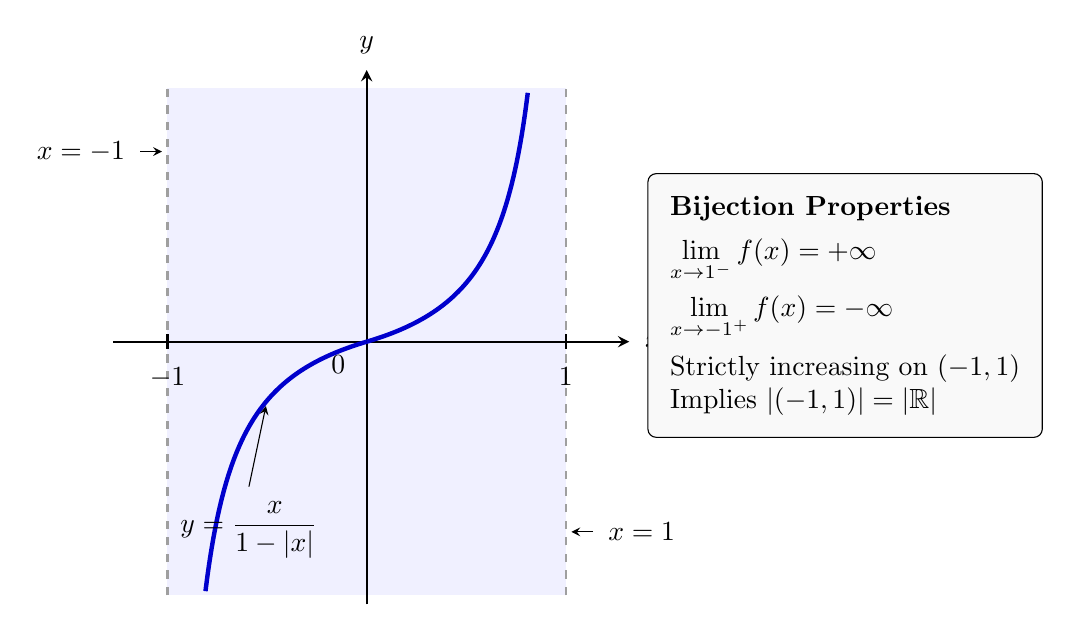
\begin{tikzpicture}[scale=1.15]
    % Layer 1: Background fill
    \fill[blue!6] (-2.2, -2.8) rectangle (2.2, 2.8);

    % Layer 2: Axes, grid lines, asymptotes, and tick marks
    \draw[dashed, gray!75, thick] (-2.2, -2.8) -- (-2.2, 2.8);
    \draw[dashed, gray!75, thick] (2.2, -2.8) -- (2.2, 2.8);
    \draw[->, >=stealth, thick, black] (-2.8, 0) -- (2.9, 0) node[right=2pt, text=black] {$x$};
    \draw[->, >=stealth, thick, black] (0, -2.9) -- (0, 3.0) node[above=2pt, text=black] {$y$};
    \draw[thick, black] (-2.2, 0.08) -- (-2.2, -0.08) node[below=3pt, text=black] {$-1$};
    \draw[thick, black] (2.2, 0.08) -- (2.2, -0.08) node[below=3pt, text=black] {$1$};
    \draw[thick, black] (0.08, 0) -- (-0.08, 0) node[below left=2pt, text=black] {$0$};

    % Layer 3: Primary plots (scaled coordinates: x_plot = 2.2*x, y_plot = 0.65*x/(1-|x|))
    \draw[ultra thick, blue!80!black, smooth, samples=80, domain=0:1.78]
        plot (\x, {0.65*\x/(2.2-\x)});
    \draw[ultra thick, blue!80!black, smooth, samples=80, domain=-1.78:0]
        plot (\x, {0.65*\x/(2.2+\x)});

    % Off-axis callouts
    \draw[->, >=stealth, shorten >=2pt, black] (-2.5, 2.1) -- (-2.2, 2.1);
    \draw[->, >=stealth, shorten >=2pt, black] (2.5, -2.1) -- (2.2, -2.1);
    \draw[->, >=stealth, shorten >=2pt, black] (-1.3, -1.6) -- (-1.1, -0.65);

    % Layer 4: Text nodes and single-node multiline annotation box
    \node[left=2pt, text=black] at (-2.5, 2.1) {$x = -1$};
    \node[right=2pt, text=black] at (2.5, -2.1) {$x = 1$};
    \node[below=2pt, text=black] at (-1.3, -1.6) {$\displaystyle y = \frac{x}{1 - |x|}$};

    \node[draw=black, fill=gray!5, rounded corners=3pt, align=left, inner sep=8pt, anchor=west, text=black]
        at (3.1, 0.4) {
            \textbf{Bijection Properties} \\[4pt]
            $\displaystyle \lim_{x \to 1^-} f(x) = +\infty$ \\[4pt]
            $\displaystyle \lim_{x \to -1^+} f(x) = -\infty$ \\[4pt]
            Strictly increasing on $(-1, 1)$ \\
            Implies $|(-1, 1)| = |\mathbb{R}|$
        };
\end{tikzpicture}
\caption{Geometric realization of the bijection $f : (-1, 1) \to \mathbb{R}$ from Theorem 11.14.}
\label{fig:bijection_plot}
\end{figure}

\subsection{Prerequisites}

Mastery of this section requires fluency in the following foundational topics:
\begin{enumerate}[label=(\arabic*)]
    \item \textbf{Proof Techniques:} Direct proof, proof by contradiction, and case analysis.
    \item \textbf{Function Theory:} Verifying injectivity ($f(a) = f(b) \implies a = b$), surjectivity ($\forall y \in B, \exists x \in A \text{ such that } f(x) = y$), and bijectivity; knowing that the inverse of a bijection is bijective (Theorem 10.15) and the composition of two bijections is bijective (Corollary 10.12).
    \item \textbf{Countability Foundations:} Properties of finite and denumerable sets, including Theorem 11.4 (every infinite subset of a denumerable set is denumerable) and the countability of $\mathbb{Z}$ and $\mathbb{Q}$.
    \item \textbf{Real Analysis and Algebra:} Solving algebraic and quadratic equations, manipulating absolute values and strict inequalities, and understanding repeating versus terminating decimal expansions.
\end{enumerate}

% ==============================================================================
% PART 2: DETAILED HOMEWORK SOLUTIONS
% ==============================================================================
\section{Detailed Homework Solutions}

In this section, we present complete, rigorous proofs for every exercise in Section 11.3.

% ------------------------------------------------------------------------------
% Exercise 11.20
% ------------------------------------------------------------------------------
\subsection{Exercise 11.20}

\textbf{Original Problem:} Prove that the set of irrational numbers is uncountable.

\textbf{Proof Technique:} Proof by Contradiction (combined with explicit bijection construction for the union of countable sets).

\begin{proof}
Let $\mathbb{I} = \mathbb{R} \setminus \mathbb{Q}$ denote the set of irrational numbers. Notice that $\mathbb{R} = \mathbb{Q} \cup \mathbb{I}$ and $\mathbb{Q} \cap \mathbb{I} = \emptyset$. We know from earlier results that the set of rational numbers $\mathbb{Q}$ is denumerable, so there exists a bijective function $f : \mathbb{N} \to \mathbb{Q}$; write $q_n = f(n)$ for each $n \in \mathbb{N}$, so that $\mathbb{Q} = \{q_1, q_2, q_3, \dots\}$ with $q_i \neq q_j$ whenever $i \neq j$.

Assume, to the contrary, that $\mathbb{I}$ is countable. By definition of a countable set, $\mathbb{I}$ is either finite or denumerable. We examine both cases and show that each implies $\mathbb{R}$ is denumerable, contradicting Corollary 11.11.

\textbf{Case 1: $\mathbb{I}$ is finite.}
First, $\mathbb{I} \neq \emptyset$ (for example, $\sqrt{2} \in \mathbb{I}$), or even if $\mathbb{I}$ has $k \ge 0$ elements, write $\mathbb{I} = \{r_1, r_2, \dots, r_k\}$ with distinct elements $r_1, \dots, r_k$ (if $k = 0$, then $\mathbb{R} = \mathbb{Q}$ is immediately denumerable). Define $h : \mathbb{N} \to \mathbb{R}$ by
\[
h(n) = \begin{cases}
r_n & \text{if } 1 \le n \le k, \\
q_{n-k} & \text{if } n > k.
\end{cases}
\]
We verify that $h$ is bijective:
\begin{itemize}
    \item \emph{Injective:} Suppose $h(m) = h(n)$ for $m, n \in \mathbb{N}$. Since $\mathbb{Q} \cap \mathbb{I} = \emptyset$, no rational number can equal an irrational number. Thus either both $m, n \le k$ or both $m, n > k$. If $m, n \le k$, then $r_m = r_n$, which implies $m = n$ because the $r_i$ are distinct. If $m, n > k$, then $q_{m-k} = q_{n-k}$, which implies $m - k = n - k$ (since $f$ is one-to-one) and hence $m = n$.
    \item \emph{Surjective:} Let $x \in \mathbb{R} = \mathbb{Q} \cup \mathbb{I}$. If $x \in \mathbb{I}$, then $x = r_i = h(i)$ for some $i \in \{1, \dots, k\}$. If $x \in \mathbb{Q}$, then since $f$ is onto, $x = q_j = h(j + k)$ for some $j \in \mathbb{N}$ with $j + k > k$.
\end{itemize}
Thus $h$ is bijective, so $\mathbb{R}$ is denumerable.

\textbf{Case 2: $\mathbb{I}$ is denumerable.}
Then there exists a bijective function $g : \mathbb{N} \to \mathbb{I}$; write $r_n = g(n)$ for each $n \in \mathbb{N}$, so $\mathbb{I} = \{r_1, r_2, r_3, \dots\}$ with $r_i \neq r_j$ for $i \neq j$. Define $h : \mathbb{N} \to \mathbb{R}$ by interleaving the two lists:
\[
h(n) = \begin{cases}
q_{(n+1)/2} & \text{if } n \text{ is odd}, \\
r_{n/2} & \text{if } n \text{ is even}.
\end{cases}
\]
We verify that $h$ is bijective:
\begin{itemize}
    \item \emph{Injective:} Suppose $h(m) = h(n)$ for $m, n \in \mathbb{N}$. Since $\mathbb{Q} \cap \mathbb{I} = \emptyset$, $h(m)$ and $h(n)$ must either both lie in $\mathbb{Q}$ (making $m, n$ both odd) or both lie in $\mathbb{I}$ (making $m, n$ both even). If $m, n$ are odd, then $q_{(m+1)/2} = q_{(n+1)/2}$; since $f$ is injective, $(m+1)/2 = (n+1)/2$, so $m = n$. If $m, n$ are even, then $r_{m/2} = r_{n/2}$; since $g$ is injective, $m/2 = n/2$, so $m = n$.
    \item \emph{Surjective:} Let $x \in \mathbb{R}$. If $x \in \mathbb{Q}$, then $x = q_k$ for some $k \in \mathbb{N}$ (since $f$ is onto), and $h(2k - 1) = q_{((2k-1)+1)/2} = q_k = x$. If $x \in \mathbb{I}$, then $x = r_k$ for some $k \in \mathbb{N}$ (since $g$ is onto), and $h(2k) = r_{2k/2} = r_k = x$.
\end{itemize}
Thus $h$ is bijective, so $\mathbb{R}$ is denumerable.

In both cases, $\mathbb{R}$ is denumerable, which implies $\mathbb{R}$ is countable. This contradicts Corollary 11.11, which states that $\mathbb{R}$ is uncountable. Therefore, our assumption is false, and the set of irrational numbers $\mathbb{I}$ is uncountable.
\end{proof}

% ------------------------------------------------------------------------------
% Exercise 11.21
% ------------------------------------------------------------------------------
\subsection{Exercise 11.21}

\textbf{Original Problem:} Prove that the set of complex numbers is uncountable.

\textbf{Proof Technique:} Direct Proof (via Theorem 11.10 and Corollary 11.11).

\begin{proof}
Recall that the set of complex numbers is defined by
\[
\mathbb{C} = \{a + bi : a, b \in \mathbb{R}, \text{ where } i^2 = -1\}.
\]
Every real number $a \in \mathbb{R}$ can be written as $a + 0i \in \mathbb{C}$, so $\mathbb{R} \subseteq \mathbb{C}$. By Corollary 11.11, the set $\mathbb{R}$ is uncountable. Applying Theorem 11.10 with $A = \mathbb{R}$ and $B = \mathbb{C}$ (since $A \subseteq B$ and $A$ is uncountable), it follows immediately that $\mathbb{C}$ is uncountable.
\end{proof}

% ------------------------------------------------------------------------------
% Exercise 11.22
% ------------------------------------------------------------------------------
\subsection{Exercise 11.22}

\textbf{Original Problem:} Prove that the open interval $(-2, 2)$ and $\mathbb{R}$ are numerically equivalent by finding a bijective function $h : (-2, 2) \to \mathbb{R}$. (Show that your function is, in fact, bijective.)

\textbf{Proof Technique:} Constructive Proof (direct verification of well-definedness, injectivity, and surjectivity by case analysis).

\begin{proof}
Define the function $h : (-2, 2) \to \mathbb{R}$ by
\[
h(x) = \frac{x}{2 - |x|}.
\]
First, observe that $h$ is well-defined: for every $x \in (-2, 2)$, we have $|x| < 2$, so $2 - |x| > 0$. Because the denominator is strictly positive, $h(x)$ is a well-defined real number for all $x \in (-2, 2)$. Moreover, the sign of $h(x)$ always matches the sign of $x$:
\begin{itemize}
    \item $h(x) = 0 \iff x = 0$,
    \item $h(x) > 0 \iff x \in (0, 2)$,
    \item $h(x) < 0 \iff x \in (-2, 0)$.
\end{itemize}

\textbf{Step 1: $h$ is one-to-one (injective).}
Let $a, b \in (-2, 2)$ and suppose that $h(a) = h(b)$, so that
\[
\frac{a}{2 - |a|} = \frac{b}{2 - |b|}.
\]
We consider three mutually exclusive cases based on the common value $h(a) = h(b)$:
\begin{itemize}
    \item \emph{Case 1: $h(a) = h(b) = 0$.} Since $2 - |a| > 0$ and $2 - |b| > 0$, the numerators must vanish, giving $a = 0$ and $b = 0$. Thus $a = b$.
    \item \emph{Case 2: $h(a) = h(b) > 0$.} Since the denominators $2 - |a|$ and $2 - |b|$ are positive, it follows that $a > 0$ and $b > 0$. Hence $|a| = a$ and $|b| = b$, so
    \[
    \frac{a}{2 - a} = \frac{b}{2 - b}.
    \]
    Cross-multiplying yields $a(2 - b) = b(2 - a)$, which expands to $2a - ab = 2b - ab$. Adding $ab$ to both sides gives $2a = 2b$, and dividing by $2$ yields $a = b$.
    \item \emph{Case 3: $h(a) = h(b) < 0$.} Since the denominators $2 - |a|$ and $2 - |b|$ are positive, we must have $a < 0$ and $b < 0$. Hence $|a| = -a$ and $|b| = -b$, so
    \[
    \frac{a}{2 + a} = \frac{b}{2 + b}.
    \]
    Cross-multiplying yields $a(2 + b) = b(2 + a)$, or $2a + ab = 2b + ab$. Subtracting $ab$ from both sides gives $2a = 2b$, and hence $a = b$.
\end{itemize}
In all three cases, $a = b$. Therefore, $h$ is one-to-one.

\textbf{Step 2: $h$ is onto (surjective).}
Let $r \in \mathbb{R}$. We exhibit an element $x \in (-2, 2)$ such that $h(x) = r$ according to the sign of $r$:
\begin{itemize}
    \item \emph{Case 1: $r = 0$.} Choose $x = 0 \in (-2, 2)$. Then $h(0) = \frac{0}{2 - |0|} = 0 = r$.
    \item \emph{Case 2: $r > 0$.} Define $x = \frac{2r}{1 + r}$. Since $r > 0$, both numerator and denominator are positive, so $x > 0$. Furthermore, since $0 < r < 1 + r$, we have $\frac{r}{1 + r} < 1$, and thus
    \[
    0 < x = \frac{2r}{1 + r} < 2,
    \]
    meaning $x \in (0, 2) \subset (-2, 2)$. Because $x > 0$, $|x| = x$, and we compute
    \[
    h(x) = \frac{\frac{2r}{1 + r}}{2 - \frac{2r}{1 + r}} = \frac{\frac{2r}{1 + r}}{\frac{2(1 + r) - 2r}{1 + r}} = \frac{2r}{2 + 2r - 2r} = \frac{2r}{2} = r.
    \]
    \item \emph{Case 3: $r < 0$.} Define $x = \frac{2r}{1 - r}$. Since $r < 0$, we have $-r > 0$, so $1 - r > 1 > 0$; thus $x < 0$. Moreover, $1 - r > -r > 0$ implies $\frac{-r}{1 - r} < 1$, which gives $-1 < \frac{r}{1 - r} < 0$, and multiplying by $2$ yields
    \[
    -2 < x = \frac{2r}{1 - r} < 0,
    \]
    meaning $x \in (-2, 0) \subset (-2, 2)$. Because $x < 0$, $|x| = -x = -\frac{2r}{1 - r}$, and we compute
    \[
    h(x) = \frac{\frac{2r}{1 - r}}{2 - \left(-\frac{2r}{1 - r}\right)} = \frac{\frac{2r}{1 - r}}{\frac{2(1 - r) + 2r}{1 - r}} = \frac{2r}{2 - 2r + 2r} = \frac{2r}{2} = r.
    \]
\end{itemize}
In every case, there exists $x \in (-2, 2)$ with $h(x) = r$. Therefore, $h$ is onto.

Since $h : (-2, 2) \to \mathbb{R}$ is both one-to-one and onto, $h$ is bijective. By definition, $(-2, 2)$ and $\mathbb{R}$ are numerically equivalent.
\end{proof}

% ------------------------------------------------------------------------------
% Exercise 11.23
% ------------------------------------------------------------------------------
\subsection{Exercise 11.23}

\textbf{Original Problem:}
\begin{enumerate}[label=(\alph*)]
    \item Prove that the function $f : (0, 1) \to (0, 2)$, mapping the open interval $(0, 1)$ into the open interval $(0, 2)$ and defined by $f(x) = 2x$, is bijective.
    \item Explain why $(0, 1)$ and $(0, 2)$ have the same cardinality.
    \item Let $a, b \in \mathbb{R}$, where $a < b$. Prove that $(0, 1)$ and $(a, b)$ have the same cardinality.
\end{enumerate}

\textbf{Proof Technique:} Direct Proof (verifying range containment, injectivity, and surjectivity of affine maps).

\begin{proof}
\textbf{Part (a):}
First, we verify that $f$ indeed maps $(0, 1)$ into $(0, 2)$. For any $x \in (0, 1)$, we have $0 < x < 1$. Multiplying all parts of the inequality by $2 > 0$ preserves the inequality direction and gives $0 < 2x < 2$, so $f(x) \in (0, 2)$.
\begin{itemize}
    \item \emph{One-to-one:} Let $x_1, x_2 \in (0, 1)$ and suppose $f(x_1) = f(x_2)$. Then $2x_1 = 2x_2$. Dividing both sides by $2$ yields $x_1 = x_2$. Hence $f$ is one-to-one.
    \item \emph{Onto:} Let $y \in (0, 2)$, so $0 < y < 2$. Set $x = \frac{y}{2}$. Dividing the inequality $0 < y < 2$ by $2 > 0$ gives $0 < \frac{y}{2} < 1$, which shows that $x \in (0, 1)$. Moreover,
    \[
    f(x) = f\!\left(\frac{y}{2}\right) = 2\left(\frac{y}{2}\right) = y.
    \]
    Hence $f$ is onto.
\end{itemize}
Since $f$ is both one-to-one and onto, $f : (0, 1) \to (0, 2)$ is bijective.

\textbf{Part (b):}
By definition, two nonempty sets $A$ and $B$ have the same cardinality if and only if there exists a bijective function from $A$ to $B$. Both $(0, 1)$ and $(0, 2)$ are nonempty sets, and in Part (a) we proved that $f : (0, 1) \to (0, 2)$ defined by $f(x) = 2x$ is a bijection. Consequently, $(0, 1)$ and $(0, 2)$ have the same cardinality, i.e., $|(0, 1)| = |(0, 2)|$.

\textbf{Part (c):}
Let $a, b \in \mathbb{R}$ with $a < b$. Note that both $(0, 1)$ and $(a, b)$ are nonempty (for instance, $\frac{1}{2} \in (0, 1)$ and $\frac{a+b}{2} \in (a, b)$). Define the function $g : (0, 1) \to (a, b)$ by
\[
g(x) = a + (b - a)x.
\]
We verify that $g$ is well-defined (maps into $(a, b)$) and bijective:
\begin{itemize}
    \item \emph{Well-definedness:} Since $a < b$, we have $b - a > 0$. For any $x \in (0, 1)$, we have $0 < x < 1$. Multiplying by the positive quantity $b - a$ yields $0 < (b - a)x < b - a$. Adding $a$ throughout gives
    \[
    a < a + (b - a)x < a + (b - a) = b,
    \]
    so $g(x) \in (a, b)$ for all $x \in (0, 1)$.
    \item \emph{One-to-one:} Let $x_1, x_2 \in (0, 1)$ and assume $g(x_1) = g(x_2)$. Then
    \[
    a + (b - a)x_1 = a + (b - a)x_2.
    \]
    Subtracting $a$ from both sides gives $(b - a)x_1 = (b - a)x_2$. Since $b - a > 0$ (in particular, $b - a \neq 0$), dividing both sides by $b - a$ yields $x_1 = x_2$. Thus $g$ is one-to-one.
    \item \emph{Onto:} Let $y \in (a, b)$, so $a < y < b$. Define
    \[
    x = \frac{y - a}{b - a}.
    \]
    Subtracting $a$ across the inequality $a < y < b$ yields $0 < y - a < b - a$. Dividing by the positive number $b - a$ gives
    \[
    0 < \frac{y - a}{b - a} < 1,
    \]
    so $x \in (0, 1)$. Evaluating $g$ at $x$ yields
    \[
    g(x) = a + (b - a)\left(\frac{y - a}{b - a}\right) = a + (y - a) = y.
    \]
    Thus $g$ is onto.
\end{itemize}
Because $g : (0, 1) \to (a, b)$ is a bijective function, the sets $(0, 1)$ and $(a, b)$ have the same cardinality.
\end{proof}

% ------------------------------------------------------------------------------
% Exercise 11.24
% ------------------------------------------------------------------------------
\subsection{Exercise 11.24}

\textbf{Original Problem:} Prove that $\mathbb{R}$ and $\mathbb{R}^+$ are numerically equivalent.

\textbf{Proof Technique:} Constructive Direct Proof (constructing an explicit exponential bijection and verifying its properties).

\begin{proof}
Here $\mathbb{R}^+ = \{y \in \mathbb{R} : y > 0\}$ denotes the set of positive real numbers. Define the function $f : \mathbb{R} \to \mathbb{R}^+$ by
\[
f(x) = e^x.
\]
For every $x \in \mathbb{R}$, $e^x$ is a strictly positive real number, so $f(x) \in \mathbb{R}^+$ and $f$ is well-defined. We prove that $f$ is bijective:
\begin{itemize}
    \item \emph{One-to-one:} Let $x_1, x_2 \in \mathbb{R}$ and suppose $f(x_1) = f(x_2)$, meaning $e^{x_1} = e^{x_2}$. Since both sides are strictly positive, we may apply the natural logarithm function $\ln : \mathbb{R}^+ \to \mathbb{R}$ to both sides, obtaining
    \[
    \ln(e^{x_1}) = \ln(e^{x_2}) \implies x_1 = x_2.
    \]
    (Equivalently, $e^x$ is strictly increasing on $\mathbb{R}$, so $x_1 \neq x_2$ implies $e^{x_1} \neq e^{x_2}$.) Hence $f$ is one-to-one.
    \item \emph{Onto:} Let $y \in \mathbb{R}^+$. Since $y > 0$, its natural logarithm $x = \ln(y)$ is a well-defined real number in $\mathbb{R}$. By the inverse property of the exponential and natural logarithm functions, we have
    \[
    f(x) = e^{\ln(y)} = y.
    \]
    Hence $f$ is onto.
\end{itemize}
Since $f : \mathbb{R} \to \mathbb{R}^+$ is bijective, $\mathbb{R}$ and $\mathbb{R}^+$ are numerically equivalent.
\end{proof}

% ------------------------------------------------------------------------------
% Exercise 11.25
% ------------------------------------------------------------------------------
\subsection{Exercise 11.25}

\textbf{Original Problem:} Consider the function $g : (-1, 1) \to \mathbb{R}$ defined by $g(x) = \frac{x}{1 - x^2}$.
\begin{enumerate}[label=(\alph*)]
    \item Prove that $g$ is onto.
    \item Prove that $g$ is one-to-one.
    \item From the information obtained in (a) and (b), what conclusion can be made?
\end{enumerate}

\textbf{Proof Technique:} Constructive Direct Proof using quadratic preimage analysis (for surjectivity) and algebraic factorization (for injectivity).

\begin{proof}
First observe that for all $x \in (-1, 1)$, we have $x^2 < 1$, so $1 - x^2 > 0$; thus $g$ is well-defined on $(-1, 1)$.

\textbf{Part (a): $g$ is onto.}
Let $r \in \mathbb{R}$. We must find an $x \in (-1, 1)$ such that $g(x) = r$. We split into two cases:
\begin{itemize}
    \item \emph{Case 1: $r = 0$.} Choose $x = 0 \in (-1, 1)$. Then $g(0) = \frac{0}{1 - 0^2} = 0 = r$.
    \item \emph{Case 2: $r \neq 0$.} Consider the candidate
    \[
    x = \frac{-1 + \sqrt{1 + 4r^2}}{2r}.
    \]
    We first show that $x \in (-1, 1)$. Because $r \neq 0$, we have $r^2 > 0$, and hence $4r^2 > 0$. This yields two strict inequalities:
    \[
    1 < 1 + 4r^2 \quad \text{and} \quad 1 + 4r^2 < 1 + 4|r| + 4r^2 = (1 + 2|r|)^2.
    \]
    Taking positive square roots gives
    \[
    1 < \sqrt{1 + 4r^2} < 1 + 2|r| \implies 0 < -1 + \sqrt{1 + 4r^2} < 2|r|.
    \]
    Dividing by $2|r| > 0$, we obtain
    \[
    0 < \frac{-1 + \sqrt{1 + 4r^2}}{2|r|} < 1.
    \]
    Since $|x| = \frac{-1 + \sqrt{1 + 4r^2}}{2|r|}$, this proves $|x| < 1$, so $x \in (-1, 1)$ (in fact, $x \in (0, 1)$ when $r > 0$ and $x \in (-1, 0)$ when $r < 0$).

    Next, we verify directly that $g(x) = r$. Computing $x^2$, we have
    \[
    x^2 = \frac{(-1 + \sqrt{1 + 4r^2})^2}{4r^2} = \frac{1 - 2\sqrt{1 + 4r^2} + (1 + 4r^2)}{4r^2} = \frac{1 + 2r^2 - \sqrt{1 + 4r^2}}{2r^2}.
    \]
    Therefore,
    \[
    rx^2 + x - r = \frac{1 + 2r^2 - \sqrt{1 + 4r^2}}{2r} + \frac{-1 + \sqrt{1 + 4r^2}}{2r} - r = \frac{2r^2}{2r} - r = r - r = 0.
    \]
    Rearranging $rx^2 + x - r = 0$ gives $x = r(1 - x^2)$. Since $x \in (-1, 1)$ ensures $1 - x^2 > 0$, dividing by $1 - x^2$ yields
    \[
    g(x) = \frac{x}{1 - x^2} = r.
    \]
\end{itemize}
Thus every $r \in \mathbb{R}$ has a preimage $x \in (-1, 1)$, proving that $g$ is onto.

\textbf{Part (b): $g$ is one-to-one.}
Let $a, b \in (-1, 1)$ and suppose $g(a) = g(b)$. Then
\[
\frac{a}{1 - a^2} = \frac{b}{1 - b^2}.
\]
Since $1 - a^2 > 0$ and $1 - b^2 > 0$, cross-multiplying yields
\[
a(1 - b^2) = b(1 - a^2) \implies a - ab^2 = b - a^2 b.
\]
Bringing all terms to the left-hand side and factoring by grouping, we obtain
\[
(a - b) + (a^2 b - ab^2) = 0 \implies (a - b) + ab(a - b) = 0 \implies (a - b)(1 + ab) = 0.
\]
Now observe that because $a, b \in (-1, 1)$, we have $|a| < 1$ and $|b| < 1$, which implies
\[
|ab| = |a| \cdot |b| < 1 \cdot 1 = 1 \implies -1 < ab < 1.
\]
Adding $1$ across this inequality yields $0 < 1 + ab < 2$. In particular, $1 + ab \neq 0$. Dividing $(a - b)(1 + ab) = 0$ by the nonzero quantity $1 + ab$ gives $a - b = 0$, so $a = b$. Hence $g$ is one-to-one.

\textbf{Part (c): Conclusion.}
From parts (a) and (b), the function $g : (-1, 1) \to \mathbb{R}$ is both onto and one-to-one; therefore, $g$ is bijective. Consequently, the open interval $(-1, 1)$ and the set $\mathbb{R}$ of real numbers are numerically equivalent (have the same cardinality), i.e., $|(-1, 1)| = |\mathbb{R}|$. Furthermore, since $\mathbb{R}$ is uncountable (Corollary 11.11), Theorem 11.13 implies that $(-1, 1)$ is also uncountable.
\end{proof}

% ==============================================================================
% PART 3: IN-DEPTH ANALYSIS OF PROBLEMS AND TECHNIQUES
% ==============================================================================
\section{In-Depth Analysis of Problems and Techniques}

\subsection{Problem Types and Logical Strategies}

Every exercise in Section 11.3 falls into one of three overarching structural categories:

\begin{description}[style=nextline, leftmargin=1.5em]
    \item[Category 1: Contradiction and Countable-Closure Proofs (Exercise 11.20)]
    \emph{Characteristics:} Proving that a subset $S$ obtained by removing a countable set from an uncountable set (such as $\mathbb{I} = \mathbb{R} \setminus \mathbb{Q}$) remains uncountable. Direct diagonalization on $\mathbb{I}$ is awkward because one must guarantee the constructed diagonal number is irrational; instead, proof by contradiction leverages the already-established uncountability of the ambient set $\mathbb{R}$.
    \emph{Strategy:} Assume $S$ is countable (covering both the finite and denumerable subcases). Construct an explicit bijection showing that the union of two disjoint countable sets ($S \cup \mathbb{Q} = \mathbb{R}$) is countable, thereby contradicting Corollary 11.11.

    \item[Category 2: Superset Monotonicity Proofs (Exercise 11.21)]
    \emph{Characteristics:} Proving that a larger mathematical structure $B$ (such as $\mathbb{C}$, $\mathbb{R}^n$, or a function space) is uncountable when it naturally embeds a known uncountable set $A$ (such as $(0, 1)$ or $\mathbb{R}$).
    \emph{Strategy:} Identify a clean subset inclusion $A \subseteq B$ (e.g., $\mathbb{R} \subseteq \mathbb{C}$ via $a \mapsto a + 0i$) where $A$ is already known to be uncountable, then invoke Theorem 11.10 directly. Note that the converse fails: an infinite subset of an uncountable set need not be uncountable (e.g., $\mathbb{Z} \subset \mathbb{R}$).

    \item[Category 3: Constructive Bijection and Algebraic Verification (Exercises 11.22, 11.23, 11.24, 11.25)]
    \emph{Characteristics:} Proving $|A| = |B|$ between two infinite sets—typically an open interval $(a, b)$ and either another open interval $(c, d)$, $\mathbb{R}$, or $\mathbb{R}^+$.
    \emph{Strategy:} Either (i) write down an explicit formula $f : A \to B$ (affine scaling for bounded-to-bounded, rational/asymptotic maps for bounded-to-$\mathbb{R}$, exponential map for $\mathbb{R}$-to-$\mathbb{R}^+$), verify well-definedness (range containment), prove $f(x_1) = f(x_2) \implies x_1 = x_2$, and invert the equation $f(x) = y$ while strictly verifying that the candidate preimage $x$ lies inside $A$; or (ii) compose previously proven bijections via Corollary 10.12.
\end{description}

\subsection{Key Analytical and Logical Manipulations}

\begin{enumerate}[label=\textbf{\arabic*.}]
    \item \textbf{Canonical Decimal Selection Avoiding Trailing $9$'s (Theorem 11.9):}
    In Cantor's diagonal proof, choosing $b_i \in \{4, 5\}$ rather than arbitrary $b_i \neq a_{ii}$ is essential. Without excluding $0$ and $9$, one could construct $b = 0.4999\cdots$ while $a_1 = 0.5000\cdots$, producing $b_1 \neq a_{11}$ yet $b = a_1$. Restricting $b_i \in \{4, 5\}$ ensures $b$ has no trailing $9$'s and no trailing $0$'s, forcing a unique decimal representation.

    \item \textbf{Disjoint Countable Interleaving (Exercise 11.20):}
    Because $\mathbb{Q}$ and $\mathbb{I}$ are disjoint, interleaving $q_1, r_1, q_2, r_2, \dots$ via parity ($n$ odd $\mapsto q_{(n+1)/2}$, $n$ even $\mapsto r_{n/2}$) immediately guarantees injectivity across the two branches, preventing cross-branch collisions.

    \item \textbf{Sign-Matched Case Splitting for Absolute Value Maps (Exercise 11.22):}
    For $h(x) = \frac{x}{2 - |x|}$, the denominator $2 - |x|$ is strictly positive on $(-2, 2)$, which locks the sign of $h(x)$ to the sign of $x$. Splitting $h(a) = h(b)$ into $= 0$, $> 0$, and $< 0$ cleanly removes the absolute value bars $|a|$ and $|b|$ before cross-multiplying.

    \item \textbf{Affine Normalization Between Open Intervals (Exercise 11.23):}
    The linear map $g(x) = a + (b - a)x$ translates the left endpoint $0 \mapsto a$ and scales the unit width $1 \mapsto b - a$. Because $b - a > 0$, multiplying inequalities by $b - a$ preserves strict bounds, cleanly establishing $0 < x < 1 \iff a < g(x) < b$.

    \item \textbf{Quadratic Root Selection and Bounding via $(1 + 2|r|)^2$ (Exercise 11.25a):}
    Inverting $g(x) = \frac{x}{1 - x^2} = r$ yields a quadratic equation $rx^2 + x - r = 0$ with two roots $\frac{-1 \pm \sqrt{1 + 4r^2}}{2r}$. To prove surjectivity onto $(-1, 1)$, one must select the `$+$' root and rigorously bound $\sqrt{1 + 4r^2}$ between $1$ and $1 + 2|r|$ so that $|x| < 1$ holds for all $r \neq 0$.

    \item \textbf{Factorization and Product Bound $|ab| < 1$ (Exercise 11.25b):}
    Rather than resorting to calculus ($g'(x) = \frac{1 + x^2}{(1 - x^2)^2} > 0$), cross-multiplying $\frac{a}{1 - a^2} = \frac{b}{1 - b^2}$ produces the purely algebraic factorization $(a - b)(1 + ab) = 0$. Using the domain constraint $a, b \in (-1, 1)$ gives $|ab| < 1$, ensuring $1 + ab > 0$ and forcing $a = b$.
\end{enumerate}

% ==============================================================================
% PART 4: CHEATSHEET, VISUALS, AND TIPS FOR SUCCESS
% ==============================================================================
\section{Cheatsheet, Visuals, and Tips for Success}

\subsection{Theorems and Cardinality Equivalences}

Table~\ref{tab:cardinality_summary} summarizes the principal theorems, canonical bijections, and cardinality results from Section 11.3.

\begin{table}[htbp]
\centering
\renewcommand{\arraystretch}{1.5}
\begin{tabularx}{\textwidth}{>{\displaystyle}l >{\displaystyle}c >{\displaystyle}X}
\toprule
\textbf{Set / Result} & \textbf{Cardinality / Relation} & \textbf{Canonical Witness or Justification} \\
\midrule
\text{Theorem 11.9: } (0, 1) & \text{Uncountable} & \text{Cantor diagonalization with } b_i \in \{4, 5\} \\
\addlinespace[4pt]
\text{Theorem 11.10: } A \subseteq B & A \text{ uncountable} \implies B \text{ uncountable} & \text{Contradiction via Theorem 11.4} \\
\addlinespace[4pt]
\text{Corollary 11.11: } \mathbb{R} & \text{Uncountable} & (0, 1) \subseteq \mathbb{R} \text{ and Theorem 11.10} \\
\addlinespace[4pt]
\text{Theorem 11.13: } A \text{ denum., } B \text{ uncount.} & |A| \neq |B| & \text{Composition } g \circ f \text{ cannot be bijective} \\
\addlinespace[4pt]
\text{Theorem 11.14: } (-1, 1) \text{ vs. } \mathbb{R} & |(-1, 1)| = |\mathbb{R}| & f(x) = \frac{x}{1 - |x|} \text{ or } g(x) = \frac{x}{1 - x^2}^{\vphantom{A}} \\
\addlinespace[4pt]
\text{Exercise 11.23(c): } (0, 1) \text{ vs. } (a, b) & |(0, 1)| = |(a, b)| & g(x) = a + (b - a)x \quad (a < b) \\
\addlinespace[4pt]
\text{Exercise 11.24: } \mathbb{R} \text{ vs. } \mathbb{R}^+ & |\mathbb{R}| = |\mathbb{R}^+| & f(x) = e^x \text{ (inverse } \ln y\text{)} \\
\addlinespace[4pt]
\text{Exercises 11.20 \& 11.21: } \mathbb{I},\ \mathbb{C} & \text{Uncountable} & \mathbb{R} = \mathbb{Q} \cup \mathbb{I};\quad \mathbb{R} \subseteq \mathbb{C} \\
\bottomrule
\end{tabularx}
\caption{Reference summary of uncountable sets and canonical bijections in Section 11.3.}
\label{tab:cardinality_summary}
\end{table}

\subsection{Set and Logic Visualization: Cantor's Diagonalization}

Figure~\ref{fig:cantor_diagonal} illustrates the exact mechanism of Theorem 11.9, demonstrating how the diagonal number $b$ is engineered to differ from every enumerated real number $a_n \in (0, 1)$ while avoiding alternate decimal representations.

\begin{figure}[htbp]
\centering
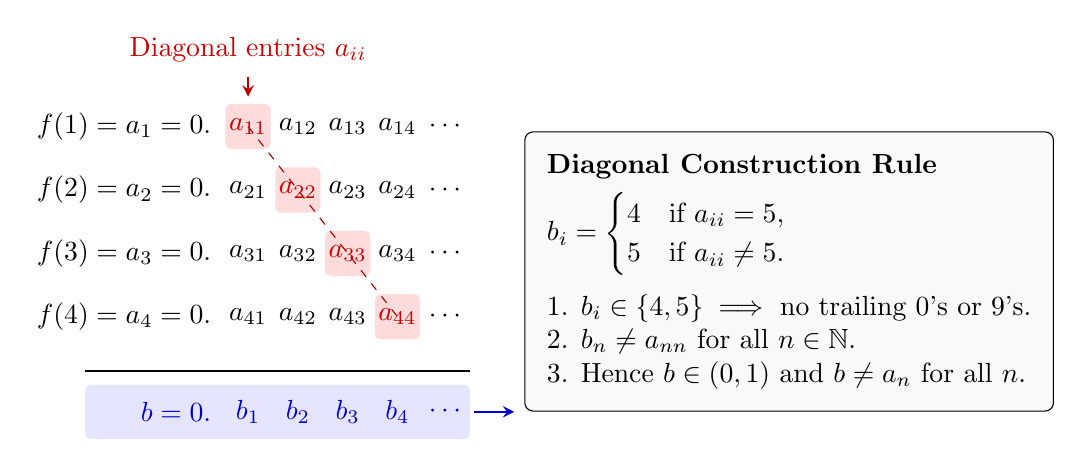
\begin{tikzpicture}[scale=1.15]
    % Layer 1: Background fills for diagonal elements
    \fill[red!14, rounded corners=2pt] (1.60, 2.75) rectangle (2.10, 3.25);
    \fill[red!14, rounded corners=2pt] (2.15, 2.05) rectangle (2.65, 2.55);
    \fill[red!14, rounded corners=2pt] (2.70, 1.35) rectangle (3.20, 1.85);
    \fill[red!14, rounded corners=2pt] (3.25, 0.65) rectangle (3.75, 1.15);
    \fill[blue!10, rounded corners=2pt] (0.05, -0.45) rectangle (4.30, 0.15);

    % Layer 2: Horizontal separator and off-axis callout arrows
    \draw[thick, black] (0.05, 0.30) -- (4.30, 0.30);
    \draw[->, >=stealth, shorten >=2pt, red!75!black, thick] (1.85, 3.55) -- (1.85, 3.27);
    \draw[->, >=stealth, shorten >=2pt, blue!80!black, thick] (4.35, -0.15) -- (4.85, -0.15);

    % Layer 3: Diagonal guide line
    \draw[dashed, red!65!black] (1.85, 3.00) -- (3.50, 0.90);

    % Layer 4: Coordinate-framed digit array and text nodes
    % Row 1
    \node[anchor=east, text=black] at (1.55, 3.00) {$f(1) = a_1 = 0.$};
    \node[text=red!80!black] at (1.85, 3.00) {$a_{11}$};
    \node[text=black] at (2.40, 3.00) {$a_{12}$};
    \node[text=black] at (2.95, 3.00) {$a_{13}$};
    \node[text=black] at (3.50, 3.00) {$a_{14}$};
    \node[text=black] at (4.05, 3.00) {$\cdots$};

    % Row 2
    \node[anchor=east, text=black] at (1.55, 2.30) {$f(2) = a_2 = 0.$};
    \node[text=black] at (1.85, 2.30) {$a_{21}$};
    \node[text=red!80!black] at (2.40, 2.30) {$a_{22}$};
    \node[text=black] at (2.95, 2.30) {$a_{23}$};
    \node[text=black] at (3.50, 2.30) {$a_{24}$};
    \node[text=black] at (4.05, 2.30) {$\cdots$};

    % Row 3
    \node[anchor=east, text=black] at (1.55, 1.60) {$f(3) = a_3 = 0.$};
    \node[text=black] at (1.85, 1.60) {$a_{31}$};
    \node[text=black] at (2.40, 1.60) {$a_{32}$};
    \node[text=red!80!black] at (2.95, 1.60) {$a_{33}$};
    \node[text=black] at (3.50, 1.60) {$a_{34}$};
    \node[text=black] at (4.05, 1.60) {$\cdots$};

    % Row 4
    \node[anchor=east, text=black] at (1.55, 0.90) {$f(4) = a_4 = 0.$};
    \node[text=black] at (1.85, 0.90) {$a_{41}$};
    \node[text=black] at (2.40, 0.90) {$a_{42}$};
    \node[text=black] at (2.95, 0.90) {$a_{43}$};
    \node[text=red!80!black] at (3.50, 0.90) {$a_{44}$};
    \node[text=black] at (4.05, 0.90) {$\cdots$};

    % Row b
    \node[anchor=east, text=blue!80!black] at (1.55, -0.15) {$b = 0.$};
    \node[text=blue!80!black] at (1.85, -0.15) {$b_1$};
    \node[text=blue!80!black] at (2.40, -0.15) {$b_2$};
    \node[text=blue!80!black] at (2.95, -0.15) {$b_3$};
    \node[text=blue!80!black] at (3.50, -0.15) {$b_4$};
    \node[text=blue!80!black] at (4.05, -0.15) {$\cdots$};

    % Callout labels
    \node[above=2pt, text=red!80!black] at (1.85, 3.55) {Diagonal entries $a_{ii}$};

    % Single-node multiline rule with anchor=west
    \node[draw=black, fill=gray!5, rounded corners=3pt, align=left, inner sep=8pt, anchor=west, text=black]
        at (4.90, 1.40) {
            \textbf{Diagonal Construction Rule} \\[4pt]
            $\displaystyle b_i = \begin{cases} 4 & \text{if } a_{ii} = 5, \\ 5 & \text{if } a_{ii} \neq 5. \end{cases}$ \\[6pt]
            1. $b_i \in \{4, 5\} \implies$ no trailing $0$'s or $9$'s. \\
            2. $b_n \neq a_{nn}$ for all $n \in \mathbb{N}$. \\
            3. Hence $b \in (0, 1)$ and $b \neq a_n$ for all $n$.
        };
\end{tikzpicture}
\caption{Cantor's diagonalization argument proving $(0, 1)$ is uncountable (Theorem 11.9).}
\label{fig:cantor_diagonal}
\end{figure}

\subsection{Heuristics and Strategic Shortcuts}

\begin{itemize}
    \item \textbf{Building New Interval Bijections by Rescaling:} Never reinvent a complicated bijection from scratch if you already know one on $(-1, 1)$ or $(0, 1)$. To map $(-R, R) \to \mathbb{R}$, replace $x$ by $x/R$ inside $\frac{x}{1 - |x|}$ to immediately obtain $h(x) = \frac{x}{R - |x|}$ (which recovers Exercise 11.22 when $R = 2$).
    \item \textbf{Choosing Between Algebraic and Calculus Proofs:} While derivatives ($f'(x) > 0$) and limits ($\lim_{x \to \pm 1^{\mp}} f(x) = \pm \infty$) quickly confirm that a candidate function is bijective during scratch work, algebraic proofs (like splitting $|x|$ into cases or factoring $(a - b)(1 + ab) = 0$) require zero calculus machinery and yield explicit inverse formulas for surjectivity.
    \item \textbf{Quick Litmus Test for Uncountability:} To show a set $S$ is uncountable, first check if $\mathbb{R} \subseteq S$ or $(a, b) \subseteq S$ (Theorem 11.10). If not, check if $S$ is the complement of a countable set inside an uncountable set (Exercise 11.20). Only use diagonalization directly when $S$ is an infinite sequence space or fractal subset (such as $\{0, 1\}^{\mathbb{N}}$ or the Cantor set).
\end{itemize}

\subsection{Common Pitfalls and Logical Fallacies}

\begin{enumerate}[label=\textbf{\arabic*.}]
    \item \textbf{The Trailing-$9$'s Decimal Fallacy:} Assuming two numbers with different $i$-th decimal digits are automatically unequal. Counterexample: $0.5000\cdots = 0.4999\cdots$ differ in \emph{every} digit position yet represent the same real number $\frac{1}{2}$.
    \item \textbf{The ``Subset of Uncountable'' Reversal Fallacy:} Confusing Theorem 11.10 ($A \subseteq B$ and $A$ uncountable $\implies B$ uncountable) with its false converse ($A \subseteq B$ and $B$ uncountable $\implies A$ uncountable). Counterexample: $\mathbb{Z} \subset \mathbb{R}$ and $\mathbb{Q} \subset \mathbb{R}$ are infinite subsets of $\mathbb{R}$, yet both are denumerable.
    \item \textbf{The Proper Subset / Geometric Length Fallacy:} Believing $|(0, 1)| < |(0, 2)|$ or $|(0, 1)| < |\mathbb{R}|$ because $(0, 1) \subsetneq (0, 2) \subsetneq \mathbb{R}$. Proper containment only implies $|A| < |B|$ for \emph{finite} sets; infinite sets routinely admit bijections onto proper subsets.
    \item \textbf{Omitting Domain Verification in Surjectivity:} Writing down an inverse algebraic expression (such as $x = \frac{-1 - \sqrt{1 + 4r^2}}{2r}$ in Exercise 11.25) without proving that $x$ actually belongs to the domain $(-1, 1)$. Only the `$+$' branch stays inside $(-1, 1)$.
\end{enumerate}

% ==============================================================================
% PART 5: CONCEPTUAL SYNTHESIS AND THE "BIG PICTURE"
% ==============================================================================
\section{Conceptual Synthesis and The ``Big Picture''}

\subsection{Thematic Connections}

The central theme unifying Section 11.3 is the \emph{decoupling of set-theoretic cardinality from geometric, algebraic, and topological size}. By defining numerical equivalence purely through the existence of a bijection, set theory strips away distance, length, order, and density:
\begin{itemize}
    \item Topologically, $(0, 1)$ is bounded with Lebesgue length $1$, whereas $\mathbb{R}$ is unbounded with infinite length; set-theoretically, Corollary 11.15 proves $|(0, 1)| = |\mathbb{R}|$.
    \item Algebraically, $\mathbb{Q}$ is dense in $\mathbb{R}$ (between any two real numbers lies a rational number), creating the illusion that rationals and irrationals are comparable in abundance. Yet $\mathbb{Q}$ is denumerable while $\mathbb{I} = \mathbb{R} \setminus \mathbb{Q}$ is uncountable (Exercise 11.20), demonstrating that the real line consists overwhelmingly of irrational (and indeed transcendental) numbers.
\end{itemize}
Together, Theorems 11.12 and 11.13 partition infinite sets into at least two fundamentally incompatible tiers: the countable infinity $\aleph_0 = |\mathbb{N}| = |\mathbb{Z}| = |\mathbb{Q}|$ and the uncountable continuum $\mathfrak{c} = |(0, 1)| = |\mathbb{R}| = |\mathbb{C}|$.

\subsection{Forward and Backward Links}

\begin{itemize}
    \item \textbf{Backward Links:} Section 11.3 directly builds upon Chapter 10's theory of functions—specifically that bijections are closed under inversion (Theorem 10.15) and composition (Corollary 10.12)—and Sections 11.1--11.2's characterization of denumerable sets and Theorem 11.4 (infinite subsets of denumerable sets are denumerable). Without those tools, proving Corollary 11.15 ($f \circ g : (0, 1) \to \mathbb{R}$ is bijective) and Theorem 11.10 would be impossible.
    \item \textbf{Forward Links:} Uncountability serves as the gateway to several major branches of higher mathematics:
    \begin{enumerate}[label=(\alph*)]
        \item \emph{Higher Cardinal Arithmetic (Sections 11.4--11.5):} Cantor's Theorem ($|A| < |\mathcal{P}(A)|$) generalizes diagonalization to prove there is no largest infinity and establishes $|\mathbb{R}| = |\mathcal{P}(\mathbb{N})| = 2^{\aleph_0}$.
        \item \emph{Measure Theory and Axiomatic Probability:} When a sample space $\Omega = [0, 1]$ or $\mathbb{R}$ is uncountable, one cannot assign a positive probability $\mathbb{P}(\{\omega\}) > 0$ to uncountably many singletons (their sum would diverge to $\infty$), nor can one consistently assign a translation-invariant measure to \emph{every} subset of $\mathbb{R}$ (the Vitali non-measurable set). Uncountability forces modern probability spaces $(\Omega, \mathcal{F}, \mathbb{P})$ to restrict events to a $\sigma$-algebra $\mathcal{F}$ (such as the Borel $\sigma$-algebra) and replace discrete summation with Lebesgue integration.
    \end{enumerate}
\end{itemize}

% ==============================================================================
% PART 6: ABSTRACT REAL-WORLD MODELING (AI, ML, & QUANT FINANCE)
% ==============================================================================
\section{Abstract Real-World Modeling in AI, Machine Learning, and Quantitative Finance}

\subsection{Concrete Scenarios}

\begin{enumerate}[label=\textbf{\arabic*.}]
    \item \textbf{Quantitative Finance: Continuous-Time Asset Pricing and Measure-Theoretic Probability:}
    In continuous-time finance (e.g., the Black--Scholes--Merton framework), stock prices take values in the uncountable space $\mathbb{R}^+$ and sample paths live in the uncountable function space $C([0, T], \mathbb{R}^+)$. Because $|\mathbb{R}^+| = |\mathbb{R}|$ (Exercise 11.24) is uncountable, every individual sample path has probability zero, and an uncountable union of measure-zero sets need not have measure zero. Consequently, risk-neutral pricing requires filtrations $(\mathcal{F}_t)_{t \in [0, T]}$ of $\sigma$-algebras and Radon--Nikodym derivatives to prevent arbitrage across uncountable state spaces.

    \item \textbf{Generative AI: Normalizing Flows and Diffeomorphic Bijections:}
    Normalizing flows transform a simple bounded or Gaussian base distribution (such as uniform noise on $(0, 1)^d$ or a standard normal on $\mathbb{R}^d$) into a complex data manifold via an explicit, invertible bijection $T : (0, 1)^d \to \mathbb{R}^d$. Just as Theorem 11.14 maps $(-1, 1) \to \mathbb{R}$ and Exercise 11.24 maps $\mathbb{R} \to \mathbb{R}^+$, neural spline and logit flows rely on smooth bijections between bounded intervals and $\mathbb{R}$ so that exact likelihoods can be evaluated through the change-of-variables Jacobian determinant.

    \item \textbf{Statistical Learning Theory: Generalization Bounds on Uncountable Hypothesis Spaces:}
    In classical PAC learning, if a hypothesis class $\mathcal{H}$ is finite (or countable with summable priors), Hoeffding's inequality combined with the union bound bounds generalization error. However, modern neural networks parametrized by $\theta \in \mathbb{R}^d$ form an \emph{uncountable} hypothesis class ($|\mathcal{H}| = |\mathbb{R}^d| = \mathfrak{c}$). A naive union bound over uncountably many hypotheses diverges, forcing Machine Learning theorists to discretize $\mathcal{H}$ via $\varepsilon$-covering numbers, VC-dimension, or Rademacher complexity.
\end{enumerate}

\subsection{Model Problem Setup: Bijective Latent-to-Asset Pricing and Normalizing Flow Framework}

We formulate a rigorous quantitative model unifying \textbf{Exercises 11.23--11.25} with \textbf{Stochastic Calculus and Generative Modeling}. Consider the problem of transforming a bounded uniform risk factor $U \in (0, 1)$ into a positive asset price $S_T \in \mathbb{R}^+$ at maturity $T > 0$ under a risk-neutral probability space $(\Omega, \mathcal{F}, \mathbb{Q})$.

\textbf{1. Spaces and Probability Measure:}
Let $(\Omega, \mathcal{F}, \mathbb{Q})$ be a complete probability space supporting a standard Brownian motion $(W_t)_{t \in [0, T]}$, where $\Omega = C([0, T], \mathbb{R})$ is uncountable and $\mathcal{F} = \mathcal{B}(\Omega)$ is the Borel $\sigma$-algebra. Let $U : \Omega \to (0, 1)$ be a uniformly distributed random variable with Lebesgue probability density $p_U(u) = \mathbf{1}_{(0, 1)}(u)$.

\textbf{2. Asset Price Dynamics (SDE):}
Under the risk-neutral measure $\mathbb{Q}$ with constant risk-free rate $r \in \mathbb{R}$ and volatility $\sigma > 0$, the asset price $S_t \in \mathbb{R}^+$ evolves according to the Geometric Brownian Motion stochastic differential equation:
\[
dS_t = r S_t \, dt + \sigma S_t \, dW_t, \qquad S_0 > 0.
\]
Applying It\^o's Lemma to $X_t = \ln S_t \in \mathbb{R}$ (which uses the bijection $\ln : \mathbb{R}^+ \to \mathbb{R}$ inverse to Exercise 11.24's map $e^x$) gives
\[
dX_t = \left(r - \frac{1}{2}\sigma^2\right) dt + \sigma \, dW_t \implies S_T = S_0 \exp\!\left(\left(r - \frac{1}{2}\sigma^2\right)T + \sigma W_T\right) \in \mathbb{R}^+.
\]

\textbf{3. Bijective Transport Map (Normalizing Flow Formulation):}
Rather than simulating $W_T$ directly, suppose a generative pricing model learns a smooth bijection $T_\theta : (0, 1) \to \mathbb{R}^+$ by composing an affine normalization $g_1(u) = 2u - 1 \in (-1, 1)$ (Corollary 11.15), an unbounded algebraic diffeomorphism $g_2(z) = \frac{z}{1 - z^2} \in \mathbb{R}$ (Exercise 11.25), a learned neural residual $\psi_\theta : \mathbb{R} \to \mathbb{R}$, and the exponential bijection $g_3(y) = e^y \in \mathbb{R}^+$ (Exercise 11.24):
\[
T_\theta(u) = \exp\!\Big(\psi_\theta\big((g_2 \circ g_1)(u)\big)\Big), \qquad u \in (0, 1).
\]
Because $g_1$, $g_2$, $\psi_\theta$ (constrained to be strictly monotone with $\psi_\theta'(\cdot) > 0$), and $g_3$ are bijections, $T_\theta : (0, 1) \to \mathbb{R}^+$ is a diffeomorphic bijection with inverse $T_\theta^{-1} : \mathbb{R}^+ \to (0, 1)$.

\textbf{4. Exact Density Evaluation and Optimization Objective:}
By the change-of-variables theorem for uncountable continuous random variables, the induced model density $q_\theta(s)$ on $\mathbb{R}^+$ is
\[
q_\theta(s) = p_U\!\big(T_\theta^{-1}(s)\big) \left|\frac{d}{ds} T_\theta^{-1}(s)\right| = \left|\big(T_\theta'\big(T_\theta^{-1}(s)\big)\big)^{-1}\right|, \qquad s \in \mathbb{R}^+.
\]
Calibrating the generative model to the risk-neutral terminal distribution $p_{S_T}$ minimizes the Kullback--Leibler divergence over the uncountable state space $\mathbb{R}^+$:
\[
\min_{\theta \in \Theta} \mathcal{L}(\theta) = \mathbb{E}_{S_T \sim p_{S_T}}\!\left[-\ln q_\theta(S_T)\right] = \int_{0}^{\infty} p_{S_T}(s) \ln\!\left|T_\theta'\!\big(T_\theta^{-1}(s)\big)\right| ds,
\]
subject to the martingale no-arbitrage constraint $\mathbb{E}_{U \sim \mathrm{Unif}(0,1)}[T_\theta(U)] = S_0 e^{rT}$.

% ==============================================================================
% PART 7: COMMON VARIATIONS AND UNTESTED CONCEPTS
% ==============================================================================
\section{Common Variations and Untested Concepts}

Several standard theorems and proof variations in advanced courses on uncountable sets do not appear in Exercises 11.20--11.25. Below are three essential omitted topics with complete, rigorous proofs.

\subsection{Closed and Half-Open Intervals Have Continuum Cardinality}

Exercise 11.23 establishes $|(0, 1)| = |(a, b)|$ for open intervals, leaving open whether adding endpoints changes cardinality.

\begin{proposition}
The closed interval $[0, 1]$ and the open interval $(0, 1)$ are numerically equivalent; that is, $|[0, 1]| = |(0, 1)|$.
\end{proposition}

\begin{proof}
Consider the countably infinite subset $C = \left\{\frac{1}{n} : n \in \mathbb{N},\, n \ge 2\right\} = \left\{\frac{1}{2}, \frac{1}{3}, \frac{1}{4}, \dots\right\} \subset (0, 1)$. We construct a bijection $f : [0, 1] \to (0, 1)$ by shifting the two endpoints $0$ and $1$ into the head of the sequence $C$ and leaving all points outside $C \cup \{0, 1\}$ fixed:
\[
f(x) = \begin{cases}
\frac{1}{2} & \text{if } x = 0, \\
\frac{1}{3} & \text{if } x = 1, \\
\frac{1}{n + 2} & \text{if } x = \frac{1}{n} \text{ for some integer } n \ge 2, \\
x & \text{if } x \in (0, 1) \setminus C.
\end{cases}
\]
First, $f(x) \in (0, 1)$ for all $x \in [0, 1]$. Next, we check bijectivity:
\begin{itemize}
    \item \emph{One-to-one:} Notice that $f(C \cup \{0, 1\}) = C$ and $f((0, 1) \setminus C) = (0, 1) \setminus C$, which are disjoint sets. On $(0, 1) \setminus C$, $f$ is the identity map, hence injective. On $C \cup \{0, 1\}$, $f$ maps distinct inputs $\{0, 1, \frac{1}{2}, \frac{1}{3}, \dots\}$ strictly to distinct outputs $\{\frac{1}{2}, \frac{1}{3}, \frac{1}{4}, \frac{1}{5}, \dots\}$. Thus $f$ is one-to-one.
    \item \emph{Onto:} Let $y \in (0, 1)$. If $y \notin C$, then $f(y) = y$. If $y = \frac{1}{2}$, then $f(0) = y$. If $y = \frac{1}{3}$, then $f(1) = y$. If $y = \frac{1}{k}$ for some integer $k \ge 4$, then $k - 2 \ge 2$ and $f\!\left(\frac{1}{k - 2}\right) = \frac{1}{k} = y$. Thus $f$ is onto.
\end{itemize}
Therefore $f : [0, 1] \to (0, 1)$ is bijective, proving $|[0, 1]| = |(0, 1)|$.
\end{proof}

\subsection{Uncountability of Infinite Binary Sequences}

While Theorem 11.9 uses base-$10$ decimals (requiring care for trailing $9$'s), diagonalization is even cleaner on the space $\{0, 1\}^{\mathbb{N}}$ of all infinite binary sequences.

\begin{proposition}
Let $B = \{ (s_1, s_2, s_3, \dots) : s_i \in \{0, 1\} \text{ for all } i \in \mathbb{N} \}$ be the set of all infinite binary sequences. Then $B$ is uncountable.
\end{proposition}

\begin{proof}
Clearly $B$ is infinite (for each $k \in \mathbb{N}$, the sequence having $1$ at index $k$ and $0$ elsewhere belongs to $B$, and all such sequences are distinct). Assume, to the contrary, that $B$ is countable; then $B$ is denumerable, so there exists a bijection $f : \mathbb{N} \to B$. Write
\[
f(n) = s^{(n)} = \big(s^{(n)}_1,\, s^{(n)}_2,\, s^{(n)}_3,\, \dots\big) \in B \qquad (n \in \mathbb{N}).
\]
Define a new binary sequence $t = (t_1, t_2, t_3, \dots) \in B$ by
\[
t_i = \begin{cases}
1 & \text{if } s^{(i)}_i = 0, \\
0 & \text{if } s^{(i)}_i = 1.
\end{cases}
\]
Because two sequences in $B$ are equal if and only if they agree in every coordinate (there is no alternate-representation ambiguity for sequences), and because $t_n \neq s^{(n)}_n$ at coordinate $n$ for every $n \in \mathbb{N}$, we have $t \neq f(n)$ for all $n \in \mathbb{N}$. Thus $f$ is not onto, contradicting the assumption that $f$ is bijective. Hence $B$ is uncountable.
\end{proof}

\subsection{Cardinality of the Plane and Complex Numbers: $|\mathbb{R}^2| = |\mathbb{R}|$}

Exercise 11.21 proves only that $\mathbb{C}$ is uncountable; an advanced follow-up shows that $\mathbb{C}$ (and $\mathbb{R}^2$) actually has the \emph{same} cardinality as $\mathbb{R}$, using the Cantor--Schr\"oder--Bernstein Theorem (which states that if there exist injections $A \to B$ and $B \to A$, then $|A| = |B|$).

\begin{proposition}
The sets $(0, 1) \times (0, 1)$ and $(0, 1)$ are numerically equivalent, and consequently $|\mathbb{C}| = |\mathbb{R}^2| = |\mathbb{R}|$.
\end{proposition}

\begin{proof}
First, the map $\phi : (0, 1) \to (0, 1) \times (0, 1)$ defined by $\phi(x) = (x, \frac{1}{2})$ is clearly injective: if $(x_1, \frac{1}{2}) = (x_2, \frac{1}{2})$, then $x_1 = x_2$.

Second, for every $x \in (0, 1)$, write its unique canonical decimal expansion $x = 0.x_1 x_2 x_3 \cdots$ that does \emph{not} end in an infinite tail of $9$'s. Define $\psi : (0, 1) \times (0, 1) \to (0, 1)$ by interleaving digits:
\[
\psi(x, y) = 0.x_1 y_1 x_2 y_2 x_3 y_3 \cdots,
\]
where $x = 0.x_1 x_2 \cdots$ and $y = 0.y_1 y_2 \cdots$ are canonical non-trailing-$9$ expansions. Note that $\psi(x, y) \in (0, 1)$ because neither $x$ nor $y$ is $0.000\cdots$ or $0.999\cdots$. Crucially, the interleaved expansion $0.x_1 y_1 x_2 y_2 \cdots$ \emph{cannot} end in an infinite tail of $9$'s: if it did, then both $(x_k)$ and $(y_k)$ would equal $9$ for all sufficiently large $k$, contradicting our canonical choice for $x$ and $y$.

Now suppose $\psi(x, y) = \psi(x', y')$. Because neither interleaved string ends in an infinite tail of $9$'s, the two numbers have identical decimal expansions digit-by-digit: $x_k = x'_k$ and $y_k = y'_k$ for all $k \in \mathbb{N}$. Hence $x = x'$ and $y = y'$, so $(x, y) = (x', y')$, proving $\psi$ is injective.

By the Cantor--Schr\"oder--Bernstein Theorem, $|(0, 1) \times (0, 1)| = |(0, 1)|$. Since there is a bijection $h : (0, 1) \to \mathbb{R}$ (Corollary 11.15), $(x, y) \mapsto (h(x), h(y))$ is a bijection from $(0, 1)^2$ to $\mathbb{R}^2$, and $(u, v) \mapsto u + vi$ is a bijection from $\mathbb{R}^2$ to $\mathbb{C}$. By composition of bijections, $|\mathbb{C}| = |\mathbb{R}^2| = |(0, 1)^2| = |(0, 1)| = |\mathbb{R}|$.
\end{proof}

% ==============================================================================
% PART 8: ADVANCED DIAGNOSTIC TESTING: "FIND THE FLAW"
% ==============================================================================
\section{Advanced Diagnostic Testing: ``Find the Flaw''}

Each of the five proofs below appears rigorous at first glance, yet contains a single, subtle, fatal mathematical or logical flaw. Identify the exact error, explain why it invalidates the proof, and supply the corrected argument.

\subsection{Diagnostic Problem 1: Modified Diagonal Digits}

\textbf{Claim:} The open interval $(0, 1)$ is uncountable.

\textbf{Flawed Proof:}
Assume to the contrary that $(0, 1)$ is countable. Since $(0, 1)$ is infinite, there is a bijection $f : \mathbb{N} \to (0, 1)$. For each $n \in \mathbb{N}$, write $f(n) = a_n = 0.a_{n1} a_{n2} a_{n3} \cdots$ using the decimal expansion that does not terminate in $9$'s. Define $b = 0.b_1 b_2 b_3 \cdots$ by setting
\[
b_i = \begin{cases}
9 & \text{if } a_{ii} \neq 9, \\
0 & \text{if } a_{ii} = 9.
\end{cases}
\]
Since $b_i \in \{0, 9\}$ for every $i \in \mathbb{N}$, we clearly have $b \in (0, 1)$. Moreover, for every $n \in \mathbb{N}$, $b_n \neq a_{nn}$, so the decimal expansion of $b$ differs from that of $a_n$ in the $n$-th position. Thus $b \neq a_n$ for all $n \in \mathbb{N}$, contradicting that $f$ is onto. Therefore $(0, 1)$ is uncountable.

\subsection{Diagnostic Problem 2: Direct Subset Proof for Irrationals}

\textbf{Claim:} The set $\mathbb{I}$ of irrational numbers is uncountable.

\textbf{Flawed Proof:}
By Corollary 11.11, the set $\mathbb{R}$ of real numbers is uncountable. The set of irrational numbers $\mathbb{I} = \mathbb{R} \setminus \mathbb{Q}$ is an infinite subset of $\mathbb{R}$ (for instance, $\{n\sqrt{2} : n \in \mathbb{N}\} \subseteq \mathbb{I}$). Since any infinite subset of an uncountable set is uncountable, it follows immediately that $\mathbb{I}$ is uncountable.

\subsection{Diagnostic Problem 3: Alternative Surjectivity Root for $g(x) = \frac{x}{1 - x^2}$}

\textbf{Claim:} The function $g : (-1, 1) \to \mathbb{R}$ defined by $g(x) = \frac{x}{1 - x^2}$ is onto.

\textbf{Flawed Proof:}
Let $r \in \mathbb{R}$. If $r = 0$, then $g(0) = 0$. Now suppose $r \neq 0$. Setting $\frac{x}{1 - x^2} = r$ gives $rx^2 + x - r = 0$. By the quadratic formula, the equation has real roots since the discriminant $1 + 4r^2 > 0$. Choosing the root
\[
x = \frac{-1 - \sqrt{1 + 4r^2}}{2r},
\]
we substitute $x$ into $rx^2 + x - r = 0$, confirming $x = r(1 - x^2)$. Because $x$ satisfies this equation, dividing by $1 - x^2$ gives $g(x) = \frac{x}{1 - x^2} = r$. Since $r \in \mathbb{R}$ was arbitrary, $g$ is onto.

\subsection{Diagnostic Problem 4: Disproving Numerical Equivalence via Length and Containment}

\textbf{Claim:} The open intervals $(0, 1)$ and $(0, 2)$ are not numerically equivalent.

\textbf{Flawed Proof:}
Assume to the contrary that $|(0, 1)| = |(0, 2)|$. Then there exists a bijection $f : (0, 1) \to (0, 2)$. Observe that $(0, 1) \subsetneq (0, 2)$ and that the interval $(0, 2)$ has geometric length $2$, whereas $(0, 1)$ has geometric length $1$. Under the natural correspondence mapping each point $x \in (0, 1)$ into $(0, 2)$, the image has length $1$, leaving the entire subinterval $[1, 2) \subset (0, 2)$ uncovered. Since $[1, 2)$ is infinite and uncovered, no bijection from $(0, 1)$ onto $(0, 2)$ can cover $[1, 2)$, contradicting that $f$ is onto. Hence $|(0, 1)| \neq |(0, 2)|$.

\subsection{Diagnostic Problem 5: Injectivity of $g(x) = \frac{x}{1 - x^2}$ on $(-2, 2) \setminus \{-1, 1\}$}

\textbf{Claim:} The function $g : (-2, 2) \setminus \{-1, 1\} \to \mathbb{R}$ defined by $g(x) = \frac{x}{1 - x^2}$ is one-to-one.

\textbf{Flawed Proof:}
Let $a, b \in (-2, 2) \setminus \{-1, 1\}$ and suppose $g(a) = g(b)$, so $\frac{a}{1 - a^2} = \frac{b}{1 - b^2}$. Because $a, b \notin \{-1, 1\}$, both denominators $1 - a^2$ and $1 - b^2$ are nonzero. Cross-multiplying gives $a(1 - b^2) = b(1 - a^2)$, which rearranges to $(a - b)(1 + ab) = 0$. Thus either $a = b$ or $ab = -1$. Suppose $ab = -1$; then $a$ and $b$ must have opposite signs (one positive, one negative). However, $g(x)$ is positive for $x > 0$ and negative for $x < 0$ near $0$, so $g(a) = g(b)$ forces $a$ and $b$ to have the same sign. Therefore $ab \neq -1$, leaving $a = b$. Hence $g$ is one-to-one.

\subsection{Solution Key}

\begin{enumerate}[label=\textbf{Flaw \arabic*:}]
    \item \textbf{Failure to Avoid $0$ and $9$ (Trailing-$9$'s and Endpoint Trap):}
    First, if $a_{ii} = 9$ for all $i \in \mathbb{N}$ (note: this cannot happen if we strictly forbid trailing $9$'s, yet $a_{ii} = 9$ can occur finitely often, or $a_{ii} \neq 9$ for all $i \in \mathbb{N}$!), then choosing $b_i = 9$ for all $i$ produces $b = 0.9999\cdots = 1 \notin (0, 1)$, violating $b \in (0, 1)$. Even more subtly, if $a_1 = 0.1000\cdots$ and $a_{nn} \neq 9$ for all $n \ge 2$ while $a_{11} = 1$, then $b_1 = 9$? Wait: if $a_1 = 0.9000\cdots$, then $a_{11} = 9 \implies b_1 = 0$, and if $a_{ii} \neq 9$ for all $i \ge 2$, then $b = 0.0999\cdots = 0.1000\cdots$. If $0.1000\cdots$ happened to be $a_2$, then $b = a_2$ even though $b_2 \neq a_{22}$!
    \emph{Correction:} Restrict $b_i$ to two digits distinct from both $0$ and $9$, such as $b_i \in \{4, 5\}$ defined by $b_i = 4$ if $a_{ii} = 5$ and $b_i = 5$ if $a_{ii} \neq 5$. Then $b \in (0, 1)$ strictly and $b$ has no trailing $0$'s or $9$'s.

    \item \textbf{False Converse of Theorem 11.10:}
    The assertion ``any infinite subset of an uncountable set is uncountable'' is false. While every infinite subset of a \emph{denumerable} set is denumerable (Theorem 11.4), an uncountable set like $\mathbb{R}$ contains denumerable infinite subsets such as $\mathbb{N}$, $\mathbb{Z}$, and $\mathbb{Q}$. Theorem 11.10 states the opposite direction: if $A \subseteq B$ and $A$ is uncountable, then $B$ is uncountable.
    \emph{Correction:} Use the proof of Exercise 11.20: write $\mathbb{R} = \mathbb{Q} \cup \mathbb{I}$, assume $\mathbb{I}$ is countable, prove $\mathbb{R}$ would then be countable, and contradict Corollary 11.11.

    \item \textbf{Choosing the Out-of-Domain Quadratic Root:}
    For $r \neq 0$, the chosen root $x = \frac{-1 - \sqrt{1 + 4r^2}}{2r}$ satisfies $|x| = \frac{1 + \sqrt{1 + 4r^2}}{2|r|} > \frac{1 + 2|r|}{2|r|} > 1$, so $x \notin (-1, 1)$ for \emph{every} $r \neq 0$! Because the proof never checked whether $x \in (-1, 1)$, it exhibited an algebraic solution outside the domain of $g$.
    \emph{Correction:} Use the other root $x = \frac{-1 + \sqrt{1 + 4r^2}}{2r}$, and prove $0 < |x| < 1$ using $1 < \sqrt{1 + 4r^2} < 1 + 2|r|$, as done in Exercise 11.25(a).

    \item \textbf{Confusing the Inclusion Map with an Arbitrary Bijection:}
    The proof conflates the identity inclusion map $\iota(x) = x$ (whose image on $(0, 1)$ misses $[1, 2)$) with an arbitrary bijection $f : (0, 1) \to (0, 2)$. Cardinality does not require preserving geometric length or using the identity map; $f(x) = 2x$ stretches $(0, 1)$ onto $(0, 2)$ and covers $[1, 2)$ via $(1/2, 1)$.
    \emph{Correction:} The claim itself is false. Prove $|(0, 1)| = |(0, 2)|$ using the bijection $f(x) = 2x$ as in Exercise 11.23(a)--(b).

    \item \textbf{Ignoring Sign Reversal of $1 - x^2$ Outside $(-1, 1)$:}
    On $(-2, 2) \setminus \{-1, 1\}$, the denominator $1 - x^2$ changes sign when $|x| > 1$! Specifically, when $x < -1$ (for instance $x = -\frac{3}{2}$), both numerator $x < 0$ and denominator $1 - x^2 < 0$ are negative, making $g(x) > 0$. Thus $g(a) = g(b) > 0$ does \emph{not} force $a$ and $b$ to have the same sign. In fact, $g$ is not one-to-one on $(-2, 2) \setminus \{-1, 1\}$: taking $a = \frac{2}{3}$ and $b = -\frac{3}{2}$ gives $ab = -1$ and
    \[
    g\!\left(\frac{2}{3}\right) = \frac{2/3}{1 - 4/9} = \frac{6}{5} \qquad \text{and} \qquad g\!\left(-\frac{3}{2}\right) = \frac{-3/2}{1 - 9/4} = \frac{6}{5}.
    \]
    \emph{Correction:} Restrict the domain to $(-1, 1)$, where $|a| < 1$ and $|b| < 1$ strictly guarantee $|ab| < 1$, so $1 + ab > 0$ and $ab = -1$ is impossible.
\end{enumerate}

\end{document}